

\documentclass{article}
\usepackage{tikz,pgfplots}
\definecolor{forestgreen}{rgb}{0.0, 0.27, 0.13}

\pagestyle{empty}
\begin{document}
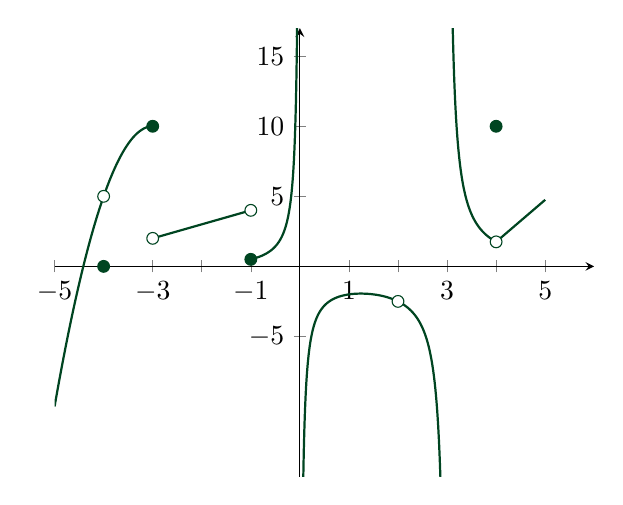
\begin{tikzpicture}
 \begin{axis}[
  axis lines=center, 
  ymin=-15, 
  xmin=-5, 
  xmax=6, 
  ymax=17, 
  no marks, 
  xtick={-5,-4,-3,-2,-1,0,1,2,3,4,5}, 
  xticklabels={$-5$,,$-3$,,$-1$,,1,,3,,5}, 
  ytick={-5,5,10,15}, 
  yticklabels={$-5$,5,10,15}, 
  ]  
    \addplot+[smooth,forestgreen, domain=-3:-.95, samples=500, thick] {x+5};
  \addplot+[smooth,forestgreen, domain=-5:-3, samples=500, thick] {-5*(x+3)^2+10};
  \addplot+[smooth,forestgreen, domain=-1:-.01, samples=500, thick] {(x+3)*(x-2)/((x-2)*(x-3)*x)};
  \addplot+[smooth,forestgreen, domain=.01:2.9, samples=500, thick] {(x+3)*(x-2)/((x-2)*(x-3)*x)};
  \addplot+[smooth,forestgreen, domain=3.1:3.95, samples=500, thick] {(x+3)*(x-2)/((x-2)*(x-3)*x)};
  \addplot+[solid,smooth,forestgreen, domain=4:5, samples=500, thick] {3*(x-4)+1.75};


  \node[circle, draw=forestgreen,fill=white,inner sep=1.5pt] at (axis cs:2,-2.5) {};
  \node[circle, draw=forestgreen,fill=forestgreen,inner sep=1.5pt] at (axis cs:-1,.5) {};
  \node[circle, draw=forestgreen,fill=white,inner sep=1.5pt] at (axis cs:-1,4) {};
  \node[circle, draw=forestgreen,fill=white,inner sep=1.5pt] at (axis cs:-3,2) {};
  \node[circle, draw=forestgreen,fill=forestgreen,inner sep=1.5pt] at (axis cs:-3,10) {};
  \node[circle, draw=forestgreen,fill=white,inner sep=1.5pt] at (axis cs:-4,5) {};
  \node[circle, draw=forestgreen,fill=white,inner sep=1.5pt] at (axis cs:4,1.75) {};
  \node[circle, draw=forestgreen,fill=forestgreen,inner sep=1.5pt] at (axis cs:-4,0) {};
  \node[circle, draw=forestgreen,fill=forestgreen,inner sep=1.5pt] at (axis cs:4,10) {};

 \end{axis}

\end{tikzpicture}
\end{document}
